\documentclass[10pt, journal]{IEEEtran}
\usepackage{amsmath}
\usepackage{amsfonts}
\usepackage{amssymb}
\usepackage{hyperref}
\usepackage{graphicx}
\graphicspath{ {images/} }
\usepackage[caption=false,font=footnotesize]{subfig}

\makeatletter
\def\endthebibliography{%
  \def\@noitemerr{\@latex@warning{Empty `thebibliography' environment}}%
  \endlist
}
\makeatother

\title{Resilience to Data Scarcity in the U-Net Architecture}

\author{Benjamin Killeen %
  \thanks{Benjamin Killeen is an undergraduate with the Department of Computer
    Science, University of Chicago, Chicago, IL 60637, USA (email:
    \href{mailto:killeen@uchicago.edu}{killeen@uchicago.edu})} %
}


\begin{document}
\maketitle

\begin{abstract}
  Deep convolutional neural networks (DCNNs) underlie myriad recent successes in
  computer vision tasks, but these successes also rely on very large, labeled
  datasets for training. In many cases, especially scientific tasks, this volume
  is untenable due to the cost of labeling. In this paper, we examine the U-Net
  architecture's resilience to data scarcity as well as the effect of various
  data augmentation schemes on its performance.\footnote{Code available at
    \href{https://github.com/bendkill/artifice}
    {github.com/bendkill/artifice}. See Appendix \ref{sec:impl-instr} for
    details.}
\end{abstract}

\section{Introduction}
\label{sec:introduction}

Large, labeled datasets like ImageNet \cite{deng_imagenet:_nodate} have enabled
DCNNs to succeed at increasingly advanced vision tasks. In 2012, Krizhevsky et
al. \cite{krizhevsky_imagenet_2012} coupled the volume of ImageNet with data
augmentation to achieve previously unseen accuracies in image
classification. When done properly, data augmentation effectively increases the
size of the dataset by transforming existing examples. However, it also has the
potential to cause overfitting, since no genuinely new examples are added. In
cases where the original dataset already exhibits marked scarcity, this risk is
amplified.

Although image classification is an impressive feat, many tasks demand higher
spatial resolution. Semantic segmentation consists of per-pixel classification,
a level of detail that greatly increases the cost of labeling. Although certain
applications justify the investment, and datasets like Microsoft's COCO
\cite{lin_microsoft_2014} continue to facilitate supervised training, many
use-cases which would benefit from DCNNs exhibit marked data scarcity. In
particular, Ronneberger et al. \cite{ronneberger_u-net:_2015} considers
applications of semantic segmentation in biomedical images, where the
specialized nature of each experiment forbids large dataset generation, but the
localization of individual structures, \textit{e.g.} neurons, in electron
microscope stacks would be invaluable. In general, scientific tasks often
exhibit this data scarcity. Ronneberger et al. addresses this problem by
introducing the U-Net architecture, which confronts data scarcity through a
combination of data augmentation and network design.

In this paper, we evaluate the performance of U-Net on the Oxford-IIIT Pet
dataset \cite{parkhi_cats_2012} under increasing levels of data scarcity. We
also examine the effect two data augmentation methods on each dataset:
horizontal flipping and random thumbnail extraction. We evaluate the
classification accuracy of U-Net on a test set consisting of $222$ examples,
withheld during training.

\section{Method}
\label{sec:method}

\begin{figure}
  \centering
  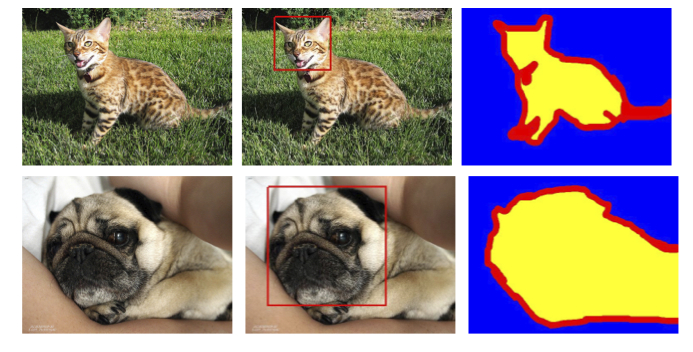
\includegraphics[width=\linewidth]{pet_annotations}
  \caption{Examples from the original Oxford-IIIT Pet Dataset
    \cite{parkhi_cats_2012}. Original images (left) are annotated with bounding
    boxes (middle) and segmentation trimaps (right).}
  \label{fig:pets}
\end{figure}

The Oxford-IIIT Pet \cite{parkhi_cats_2012} dataset consists of $7349$ images of
individual cats and dogs. There are 37 different breeds represented, with
approximately $200$ examples from each breed. For simplicity, we limited our
classification to three classes: cat, dog, and background, but in every dataset,
we retained as much uniformity as possible across breeds. The testing set, for
example, consists of $n_{\text{test}} = 6$ examples from each breed. We also
resized each image to $512 \times 512$, for uniformity. As shown in
Fig. \ref{fig:pets}, the Pet dataset includes bounding boxes and semantic
segmentation trimaps. To recover labels, we remap the boundary region of each
trimap to the animal's classification, and resize the resulting annotation to
$512\times 512$, correcting misclassification from interpolation as necessary.

In order to observe the effect of increasing data scarcity $S$, we generate four
datasets with $S = 0, 0.3, 0.6$, and $0.9$. $S$ determines the number of
examples drawn from each breed $N_{b,S}$ according to
\[ N_{b,S} = \lfloor(1 - S) \cdot (N_b - n_{\text{test}})\rfloor, \] where $N_b$
is the number of examples from breed $b$ in the original dataset. Table
\ref{tab:dataset-summary} shows the resulting number of examples in each
generated dataset, for different scarcity levels.

In addition to examining increasing scarcity, we examine the effects of two
augmentation schemes. The first augmentation, ``flip,'' consists of flipping the
image horizontally. Applying the same transformation to the annotation results
in a ``new'' labeled example. Applying just this transformation doubles the size
of the dataset. The second augmentation, ``thumbnail,'' extracts a random
$384\times 384$ subsection from the original image and resizes it to
$512\times 512$ (extracting the same subsection from the annotation). We apply
the ``thumbnail'' augmentation with the ``flip'' augmentation additively,
tripling the size of the original dataset. Table \ref{tab:dataset-summary} shows
the number of examples in each augmented dataset, at each scarcity level.

\begin{figure}
  \centering
  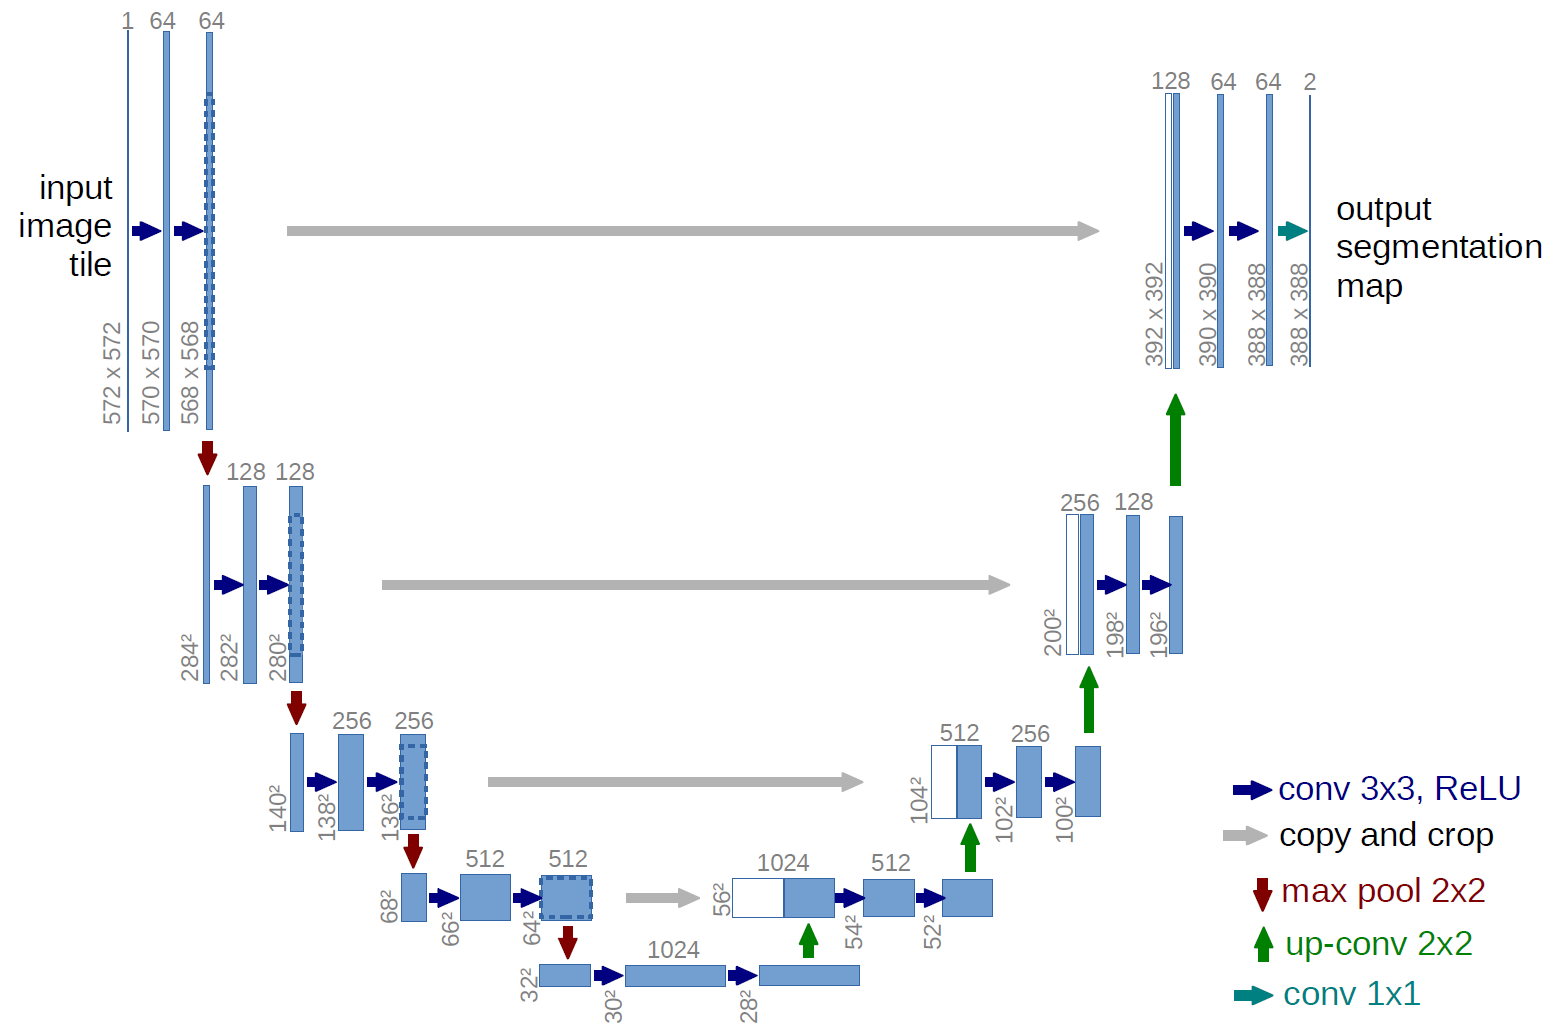
\includegraphics[width=\linewidth]{u-net-architecture}
  \caption[unet]{The U-Net architecture \cite{ronneberger_u-net:_2015}. Blue
    boxes correspond to muli-channel feature maps. White boxes represent copied
    feature maps. Arrows represent various operations.}
  \label{fig:unet}
\end{figure}

\subsection{Model}
\label{sec:model}

Fig. \ref{fig:unet} describes the U-Net architecture, which uses a series of
convolutions and ``de-convolutions'' or ``up-convolutions'' to build up abstract
feature maps at multiple levels while maintaining high spatial resolution for
the final segmentation. We implement this architecture using Tensorflow
\cite{abadi_tensorflow:_nodate}, and for each experiment limit training to one
epoch.\footnote{Results from time constraints. In future experiments, we aim to
  evaluate U-Net's performance over many epochs.} With a batch size of four, we
utilize Adam optimization \cite{kingma_adam:_2014} over pixel-wise cross-entropy
between predicted and ground-truth annotations.

\section{Results}
\label{sec:results}

We evaluate the performance of U-Net in terms of the average test-accuracy
across all pixels. Table \ref{tab:dataset-summary} shows the results of training
for one epoch on each dataset, measuring the performance on a separate test set
withheld during training. Firstly, we note the marked decline in accuracy as
scarcity increases (with no augmentations). Training with $S = 0$ yields an
accuracy of 73.6\% (compare to random classification 33\%). We believe that
further epochs would significantly improve this value. The smallest dataset, by
contrast, yielded an accuracy of only 58.9\%.

As can be seen, the effects of augmentation are most significant for datasets
with high scarcity. The $S = 0.9$ set saw a 7.3\% increase in accuracy after
applying both augmentations. The $S = 0$ dataset, by contrast, only experienced
a 3.1\% increase with the ``flip'' augmentation, and applying both augmentations
actually caused some overfitting, decreasing the accuracy compared to just
``flip.''

\begin{table}
  \centering
  \begin{tabular}{|c|c|c|c|}
    \hline
    Scarcity & Augmentations & Examples & Test Accuracy (\%) \\
    \hline
    0 & None & 7128 & 73.6 \\
    \hline
    0 & flip & 14256 & 76.7 \\
    \hline
    0 & flip, thumbnail & 21384 & 75.2 \\
    \hline
    0.3 & None & 4960 & 73.1 \\
    \hline
    0.3 & flip & 9916 & 75.1 \\
    \hline
    0.3 & flip, thumbnail & 14876 & 75.7 \\
    \hline
    0.6 & None & 2824 & 70.4 \\
    \hline
    0.6 & flip & 5648 & 73.8 \\
    \hline
    0.6 & flip, thumbnail & 8472 & 74.4 \\
    \hline
    0.9 & None & 664 & 58.9 \\
    \hline
    0.9 & flip & 1324 & 63.6 \\
    \hline
    0.9 & flip, thumbnail & 1988 & 66.2 \\
    \hline
  \end{tabular}
  \vspace{0.7em}
  \caption{}
  \label{tab:dataset-summary}
\end{table}

\section{Discussion}
\label{sec:discussion}

We have shown the effects of increasing data scarcity on the U-Net architecture,
as well as the improvements that can be made through simple data
augmentation. Although these results are promising, we recognize that much work
remains to be done. For instance, we have made the choice (due to time
constraints) to limit training to one epoch. While practical, this decision
results in a fundamental ambiguity between the effects of data scarcity, where
the number unique examples decreases, and limited training.  In order to more
properly measure the effects of data scarcity, it seems, U-Net should undergo a
constant number of training steps, preferably for many epochs, independent of
the number of unique examples.

In addition to this shortcoming, we were disappointed to not be able to explore
further data augmentation methods, as well as various combinations of each of
these augmentations. In particular, we wished to test the effects of object
extraction, which would use the known segmentation to extract a cat or dog from
the image, translate it within the image, and reinsert it. More than any other
data augmentation method, we believe this ``extract and shift'' scheme has the
potential to explore new regions of the data space. That is, it could create the
most novel examples for the network to learn from.

\bibliographystyle{IEEEtran}
\bibliography{vision_project}

\appendices{}

\section{Implementation Instructions}
\label{sec:impl-instr}

Because the implementation underlying this report is part of a larger project,
we provide instructions here for implementation validation on the University of
Chicago \verb|midway| cluster. To set up:

\begin{enumerate}
\item \verb|ssh| into \verb|midway2.rcc.uchicago.edu|.
\item Clone the repository at
  \href{https://github.com/bendkill/artifice}{github.com/bendkill/artifice}, and
  change into its root directory.
\item Run
\begin{verbatim}
export PYTHONPATH=$PYTHONPATH:`pwd`
\end{verbatim}
\item Download the Oxford-IIIT Pet dataset from
  \href{http://www.robots.ox.ac.uk/~vgg/data/pets/}{here}, and untar both
  annotations and images in \verb|data/pets|.
\item Load the compute node by running
\begin{verbatim}
sinteractive --partition=gpu2 \
  --gres=gpu:1 --mem=32000
\end{verbatim}

\item Load the environment by running
\begin{verbatim}
module load cuda/9.0
module load Anaconda3/5.0.1
source activate DL_GPU_cuda_9.0
\end{verbatim}
\item Run
\begin{verbatim}
python test_utils/pets.py -h
\end{verbatim}
  to see test installation and see options. It is normal for this to take a
  while the first time, as tensorflow sets up its environment. Some warnings are
  also normal.
\end{enumerate}

You can also run premade batch scripts for training in the \verb|batch|
directory. These may have to be modified with the proper account.

\end{document}
%%% Local Variables:
%%% mode: latex
%%% TeX-master: t
%%% End:
